\documentclass[a4paper]{article}
\usepackage[english, mongolian]{babel}
\usepackage[utf8x]{inputenc}
\usepackage{graphicx}
\usepackage{listings, paralist}
\usepackage{xcolor}
\usepackage{float}
\usepackage{url}
\usepackage{amsmath}
\usepackage{amstext}
\usepackage{amssymb}
\usepackage{multirow}
\usepackage{multicol}
\usepackage{titlesec}
\usepackage{geometry}
\usepackage{indentfirst}
\usepackage{booktabs}
\usepackage{adjustbox}
\usepackage{dblfloatfix}
\usepackage{mdframed}
\usepackage[tc]{titlepic}
\usepackage{pythonhighlight}
\usepackage[
    backend=biber,
    style=ieee
]{biblatex}
\addbibresource{citation.bib}

\tolerance=1
\emergencystretch=\maxdimen
\hyphenpenalty=10000
\hbadness=10000

\geometry{
  left=2cm, % Adjust the left margin
  right=2cm, % Adjust the right margin
  top=2cm, % Adjust the top margin
  bottom=2cm, % Adjust the bottom margin
}
\setlength{\columnsep}{0.8cm}
\setlength{\columnwidth}{\dimexpr(\linewidth-\columnsep)/2}
\fontsize{10pt}{12pt}\selectfont
\titleformat{\section}[block]{\bfseries}{\thesection.}{1em}{} 
\titleformat{\subsection}[block]{\hspace{2em}}{\thesubsection}{1em}{}

\title{Хэв танилтын үндэс Лаборатори 2-1 тайлан}
\author{Эрдэнэ Тэмүүжин - 20B1NUM1970}
\date{\today}
\begin{document}
% ----------------------------------------------------------------
\begin{titlepage}
\begin{center}
 {\huge\bfseries Хэв танилтын үндэс \\ Лаборатори 2-1 тайлан\\}
 % ----------------------------------------------------------------
 \vspace{1.5cm}
 {\Large\bfseries Эрдэнэ Тэмүүжин}\\[5pt]
 20b1num1970@stud.num.edu.mn\\[14pt]
  % ----------------------------------------------------------------
 \vfill
 % ----------------------------------------------------------------

\includegraphics[width=0.19\textwidth]{logo_web.jpg}\\[5pt]
\Large
ХШУИС Хэрэглээний Математикийн тэнхим\\
Монгол Улсын Их Сургууль\\
\vfill
{2023 оны 10-р сарын 12}
\end{center}
\end{titlepage}
% ----------------------------------------------------------------
\maketitle
\begin{center}
    \vspace{-1em}
    МУИС-ХШУИС Хэрэглээний Математикийн тэнхим \\
\end{center}
\section*{\centerline{Удиртгал}}
Энэ лабораторийн ажилд дижитал зургийн пиксел утгуудын эрчмийг өөрчлөх (Intensity Resolution), Интерполяцийн арга ашиглан зургийн мэдэгдэхгүй утгуудыг тооцох (Image Interpolation), зургийн пиксел утгуудын далайцыг сунгах (Contrast Stretching), зургийн пиксел утгуудын сонирхсон завсрын утгуудыг ихэсгэх (Gray level slicing) болон зургийн шахахад ашиглагдах арга (Bit-plane Slicing) туршсан.
\section{Intensity Resolution}
Зургийн нарийвчлал (intensity) нь зургийн пикселийг хэдэн битээр тодорхойлж байгаахаас хамаардаг. Жишээ нь хар цагаан зургийн хувьд пиксел бүрийг 1-бит буюу 0 эсвэл 1 гэсэн тоогоор илэрхийлж чадна. Харин 2-бит зурагны хувьд пиксел бүрийг нийт 4 янзаар илэрхийлж болно. 00 - хар, 11 - цагаан, 01 - бараан саарал, 10 - цайвар саарал гэсэн сонголтууд байна. 
\begin{figure}[H]
  \centering
  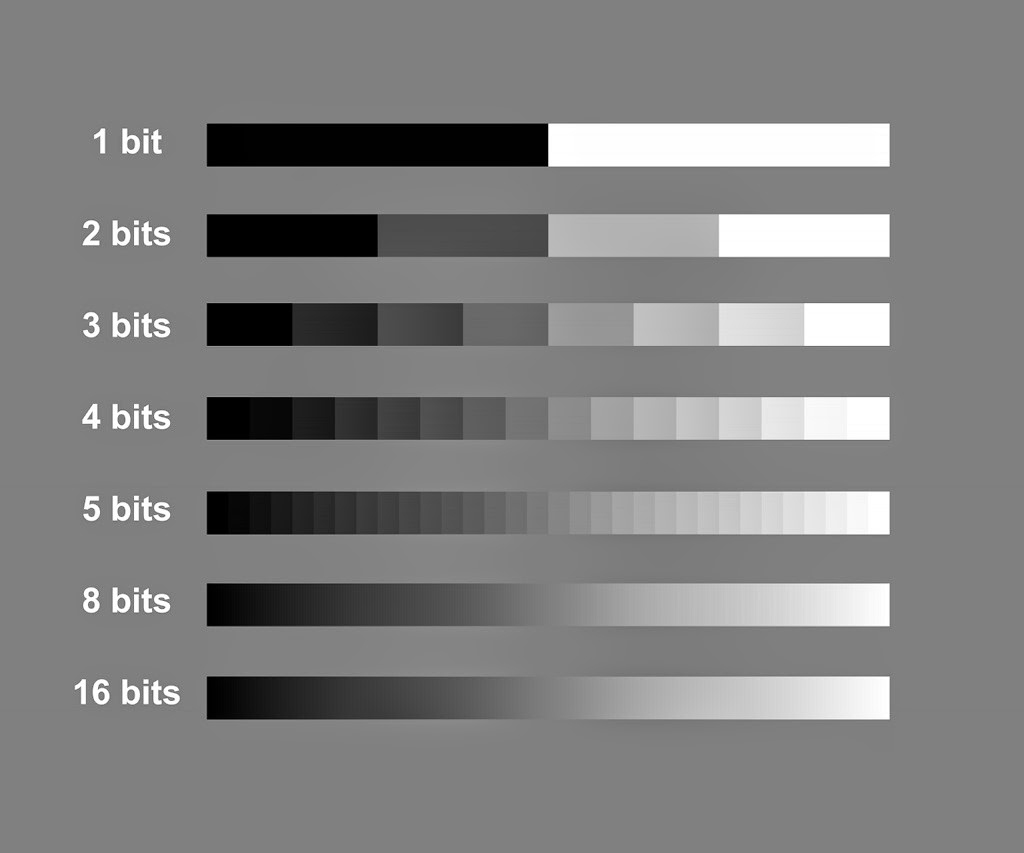
\includegraphics[scale = 0.20]{bitdepths_chart_med_1.jpg}
  \caption[Wider Face]{Зургын бит гүн \cite{bitdepth}}
\end{figure}
Энэ хэсгийн даалгавар нь анхны зураг болох 8-бит, саарал зурагийн пикселийг 1-бит хүртэл багасгах юм.
\begin{python}
a = 0
b = 255

def func(img, k):
    row, col = img.shape
    out_img = np.zeros((row, col))

    c = 0
    d = 2**k

    mult = (d - c)/(b - a)

    for i in range(row):
        for j in range(col):
            out_img[i][j] = img[i][j]*mult

    return np.uint8(out_img), c, d - 1
\end{python}
Анхны буюу 8-бит зургын пиксел бүр $p_{ij} \in \interval[{0, 255}]$ завсраас утгаа авдаг. Зургыг 7-битээр илэрхийлэхийн тулд $\hat{p}_{ij}\in\interval[{0, 127}]$ харин 6-бит $p_{ij} \in \interval[\hat{p}_{ij}\in{0, 127}]$ гэх мэтчилэн хувиргалтуудыг хийх шаардлагатай. Иймд $\hat{p}_{ij} = f(p_{ij}) = c + (\frac{d - c}{b - a})(p_{ij} - a)$ Функц зарлаж зургийг илэрхийлэх битийн хэмжээг өөрчилсөн. Энд бит бүрийн хувьд пикселийн доод утга $c = a = 0$ тул функцийг дараахаар тодорхойлсон:
\begin{equation}
    \hat{p}_{ij} = f(p_{ij}) = p_{ij}\frac{d - c}{b - a}
\end{equation}
Энд $d = 2^k$ буюу пикселийн бит, $b = 255$ 8-бит зургын пикселийн авах боломжтой утгын тоо.
\begin{figure}[H]
  \centering
  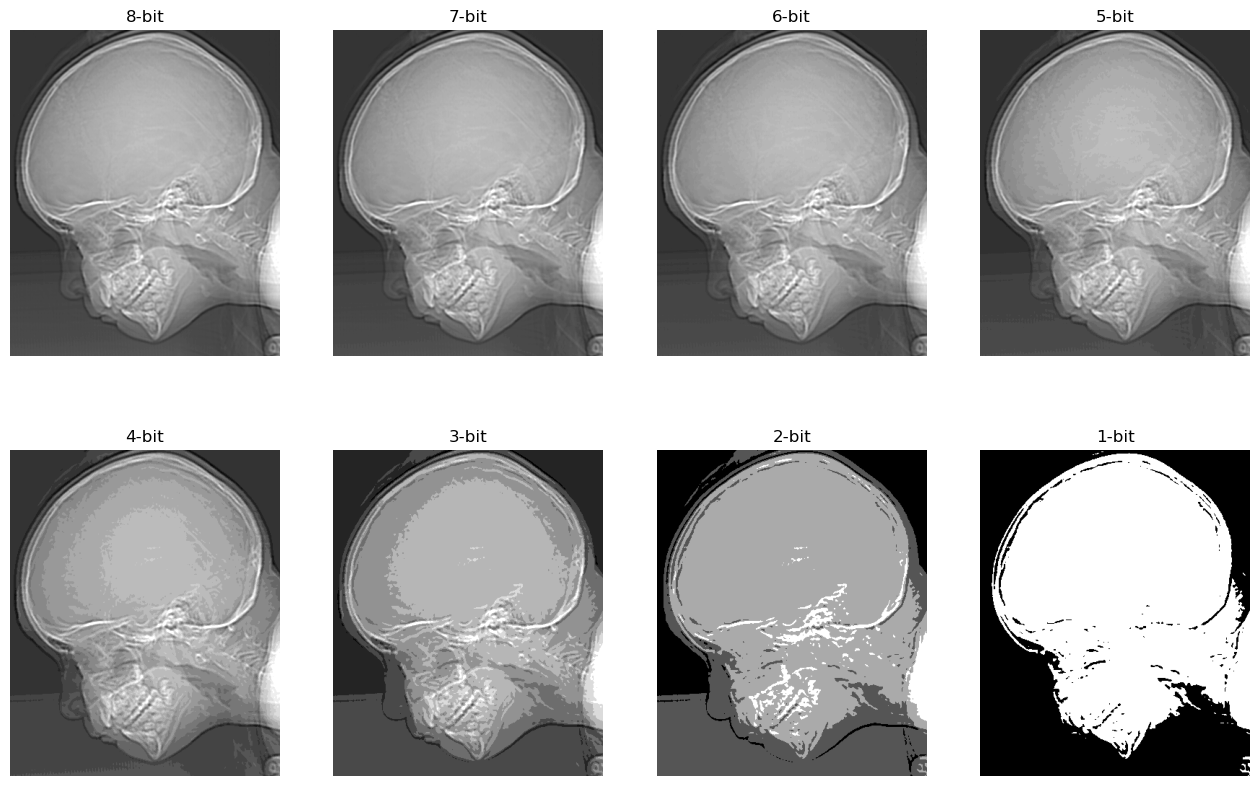
\includegraphics[scale = 0.35]{bit_depth.png}
  \caption[Wider Face]{Image Resolution үр дүн}
\end{figure}
\section{Image Interpolation}
$Q_{11} = (x_1, y_1), Q_{12} = (x_1, y_2), Q_{21} = (x_2, y_1), Q_{22} = (x_2, x_2)$ цэгүүд дээрх функцийн утгыг мэддэг гэе.
Хэвтээ тэнхлэгийн дагуу шугаман интерполяци хийнэ.
\begin{equation}
\begin{aligned}
  f(x, y_1) = \frac{x_2 - x}{x_2 - x_1}f(Q_{11}) + \frac{x - x_1}{x_2 - x_1}f(Q_{21}) \\
  f(x, y_2) = \frac{x_2 - x}{x_2 - x_1}f(Q_{12}) + \frac{x - x_1}{x_2 - x_1}f(Q_{22})
\end{aligned}
\end{equation}
\begin{figure}[H]
  \centering
  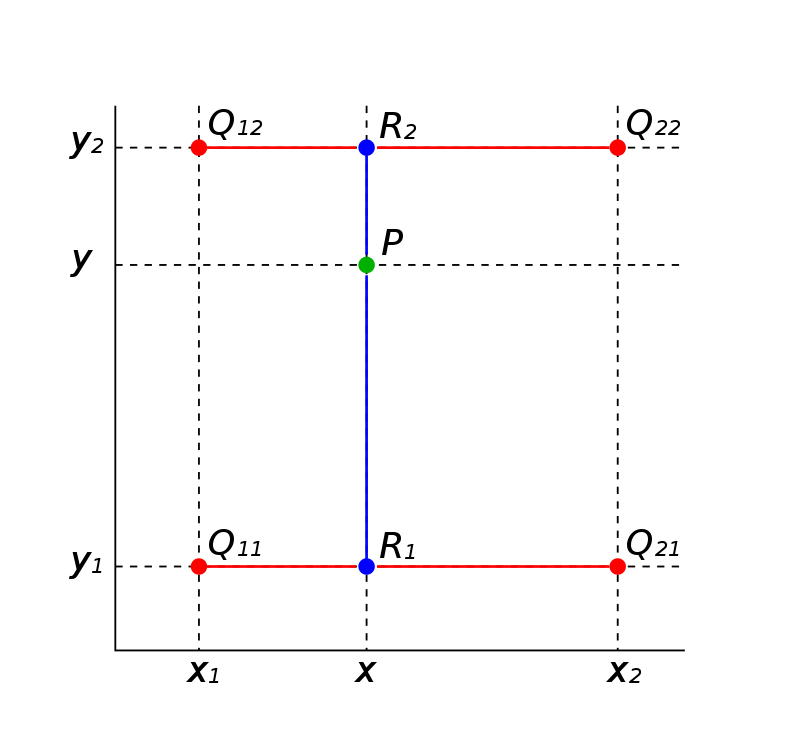
\includegraphics[scale = 0.25]{BilinearInterpolationV2.png}
  \caption[Wider Face]{Bilinear Interpolation \cite{Swienegel}}
\end{figure}
Эндээс босоо тэнхлэгийн дагуу шугаман интерполяци ашигласны дараагаар дараах ойролцооллын функцыг гаргана.
\begin{equation}
    f(x, y) = \frac{1}{(x_2 - x_1)(y_2 - y_1)}\begin{bmatrix}x_2 - x & x - x_1\end{bmatrix}\begin{bmatrix}f(Q_{11} & f(Q_{12})\\f(Q_{21} & f(Q_{22})\end{bmatrix}\begin{bmatrix}y_2 - y\\y-y_1\end{bmatrix}
\end{equation}

\begin{python}
# Nearest Neighbor Interpolation
img_128_nearest = cv2.resize(img, (128, 128), 
                             interpolation = cv2.INTER_NEAREST)
img_64_nearest = cv2.resize(img, (64, 64), 
                            interpolation = cv2.INTER_NEAREST)
img_32_nearest = cv2.resize(img, (32, 32), 
                            interpolation = cv2.INTER_NEAREST)

# Bilinear Interpolation
img_128_linear = cv2.resize(img, (128, 128), 
                            interpolation = cv2.INTER_LINEAR)
img_64_linear = cv2.resize(img, (64, 64), 
                           interpolation = cv2.INTER_LINEAR)
img_32_linear = cv2.resize(img, (32, 32), 
                           interpolation = cv2.INTER_LINEAR)
\end{python}

\begin{figure}[H]
  \centering
  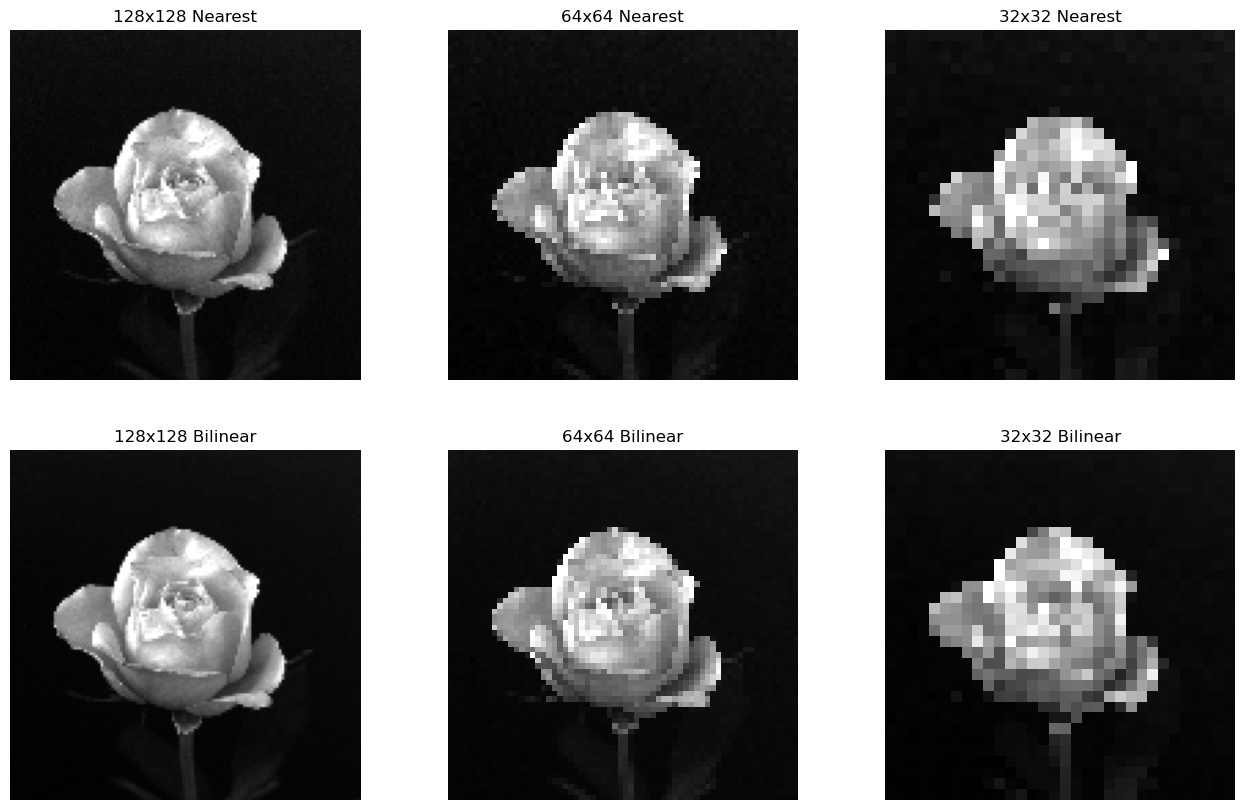
\includegraphics[scale = 0.35]{interpolation.png}
  \caption[Wider Face]{Image Interpolation үр дүн}
\end{figure}
\section{Contrast Stretching}
\section{Gray-level Slicing}
\begin{python}
h, w = img.shape
img1 = np.zeros((h, w),dtype = 'uint8')

min_range = 165
max_range = 190
range_val = 255
const_val = 45
X = []
y = []

for i in range(h):
    for j in range(w):
        if(img[i, j] >= min_range and img[i, j] <= max_range):
            img1[i, j] = range_val
            X.append(img[i, j])
            y.append(range_val)
            
        else:
            img1[i, j] = const_val
            X.append(img[i, j])
            y.append(const_val)
\end{python}
\begin{figure}[H]
  \centering
  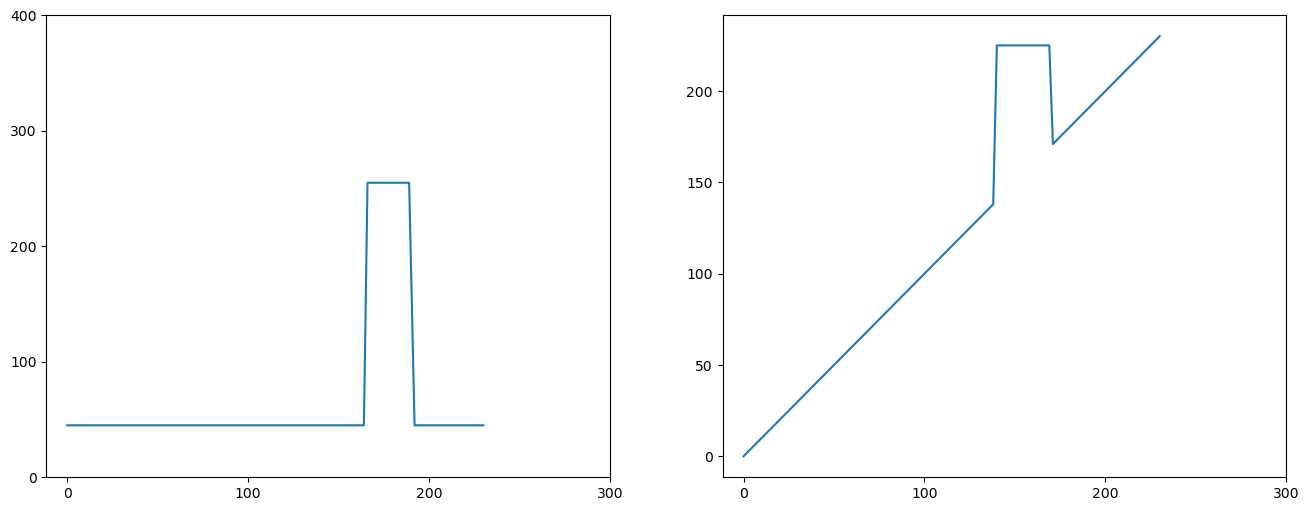
\includegraphics[scale = 0.35]{gray_level_slicing.png}
  \caption[Wider Face]{Image Interpolation үр дүн}
\end{figure}
\begin{python}
img2 = np.zeros((h, w), dtype = 'uint8')

min_range = 140
max_range = 170
range_val = 225

X2 = []
y2 = []

for i in range(h):
    for j in range(w):
        if(img[i, j] >= min_range and img[i, j] <= max_range):
            img2[i, j] = range_val
            X2.append(img[i, j])
            y2.append(range_val)
        elif(img[i, j] < min_range or img[i, j] > max_range):
            img2[i, j] = img[i, j]
            X2.append(img[i, j])
            y2.append(img[i, j])
\end{python}
Хувиргалтын функц
\begin{figure}[H]
  \centering
  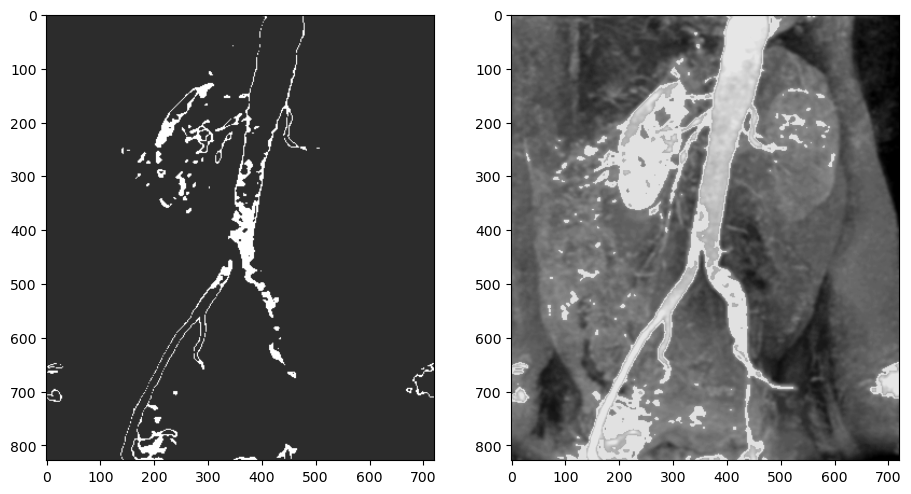
\includegraphics[scale = 0.35]{gray_level_slicing_output.png}
  \caption[Wider Face]{Image Interpolation үр дүн}
\end{figure}
\section{Bit-plane Slicing}
\section{Дүгнэлт}
\section{Ном зүй}
\printbibliography[heading=none]
\end{document}